\documentclass[10pt]{elegantbook}

\title{Large Language Model}
\subtitle{Can J.A.R.V.I.S becomes reality?}

\author{occupymars}
\date{June. 23, 2025}
\version{0.1}

\cover{iron_man.jpg}

% all the packages included
\usepackage{cprotect}
\usepackage{fontawesome}
\usepackage[linesnumbered, ruled]{algorithm2e}
\RestyleAlgo{algoruled}

% set some fonts
\setmonofont{Ubuntu Mono}

% my own commands
% \newcommand{\mydefination}[1]{\textit{\textcolor[RGB]{0,174,247}{#1}}}
\newcommand{\mydefination}[1]{\textbf{\textit{\textcolor{structurecolor}{#1}}}}

\begin{document}

\maketitle

\frontmatter
\tableofcontents

\mainmatter

\chapter{Survey}

\section{Large Language Models: A Survey}

\begin{introduction}
    \item Early Pretrained Large Language Models
    \item Large LLMs
    \item LLM Techniques
    \item Datesets
    \item Benchmarks
    \item Challenges and Future
\end{introduction}

More details please refre to \href{https://arxiv.org/abs/2402.06196}{Large Language Models: A Survey}.

\subsection{Introduction}
Statistical language model are not good because of the data sparsity, early neural language model are task specific.

Large language model have emergent abilities: \mydefination{in-context learning}, where LLMs learn a new task from a small 
set of examples presented in the prompt at inference time; \mydefination{instruction following}, where
LLMs, after instruction tuning, can follow the instructions for new types of tasks without using explicit examples;
\mydefination{multi-step reasoning}, where LLMs can solve a complex task by breaking down that task into intermediate 
reasoning steps.

\begin{figure}[htbp]
    \centering
    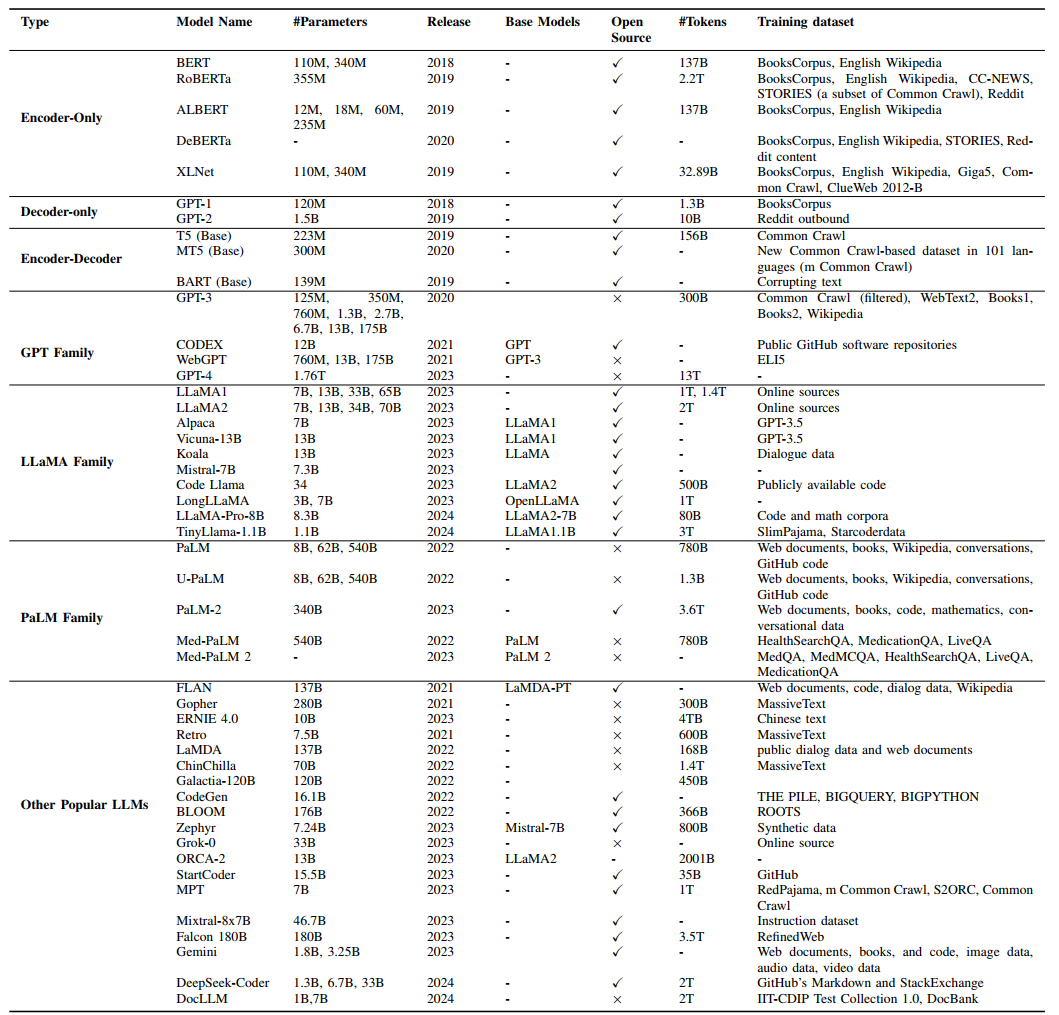
\includegraphics[width=0.90\textwidth]{image/LLM_overview.png}
    \caption{LLM Overview}
    \label{fig:LLM_overview}
\end{figure}

\subsection{Large Language Models}
First let us walk through early pre-trained neural language models. 

\begin{itemize}
    \item The first category is encoder-only models, represented by BERT.
    \begin{enumerate}
        \item BERT, pre-trained by two tasks: \mydefination{masked language modeling} (MLM) and \mydefination{next sentence
    prediction} (NSP)
        \item RoBERTa, remove NSP, train with much larger mini-batches and learning rates.
        \item ALBERT, from $V \times H$ to $V \times E \rightarrow E \times H$ by adding a linear layer, so the embedding layer 
    will has a smaller param size. 24 layers are shared (but the computation speed is same). And new NSP, instead of randomly 
    choose next sequence, inverse the true sequence pair order.
        \item DeBERTa (Decodingenhanced BERT with disentangled attention), use \mydefination{disentangled attention} compute 
    the content and position seperately; At fine-tune stage, add absolute position into decoding layer to predict masked tokens,
    enhance the MLM; Introduce a novel pre-training task, ELECTRA, known as \mydefination{replace token detection} (RTD), instead
    of mask the word, we replace it with plausible alternatives sampled from a small generated model. And pre-training will try
    to distinguish whether tokens are replaced or not. RTD is more sample-efficient than MLM because the former
    is defined over all input tokens rather than just the small subset being masked out.
        \item XLMs, 3 pre-training method, casual language model (CLM) for warmup and basic ability; MLM, shared BPE between
    different language; Translation Language Modeling (TLM), [CLS] ENGLISH [SEP] FRANCH [SEP] with mask.
        \item XLNet, based on Transformer-XL, utilize auto-regressive (decoder), use PLM (permutation language model) to 
    permutate the tokens of a sequence, use AR to predict it (only predict last $K$ tokens) so it can get bidirection information,
    then use a two stream attention because PLM make the position a problem to handle.
        \item UNILM, shared Transformer but three pre-training method, AR, AE (encoder only), seq2seq (encoder-decoder), using 
    different masks to control the context the prediction is conditioned on.
    \end{enumerate}

    \item Second category is decoder-only models, represented by GPT.
    \begin{enumerate}
        \item GPT-1, next token prediction
        \item GPT-2, Layer normalization is moved to the input of each sub-block, additional layer normalization is added
after the final self-attetion block.
    \end{enumerate}

    \item Last category is encoder-decoder PLMs, represented by T5.
    \begin{enumerate}
        \item T5 and mT5 (multilingual variance of T5).
        \item MASS (MAsked Sequence to Sequence pre-training), mask several consecutive tokens as input, decoder predicts
the masked fragment, so it jointly trains language embedding and generation.
        \item BART, it is pre-trained by corrupting text with an arbitrary noising function, and then learning to reconstruct
the original text.
    \end{enumerate}
\end{itemize}

Then we comes to LLM family.
\begin{itemize}
    \item GPT Family
    \begin{enumerate}
        \item GPT-3, maybe the first LLM, with 175B parameters, the first to show in-context learning ability (one of the emergent ability).
        \item CODEX, based on GPT-3, fine-tuned on GitHub, powers Copilot.
        \item WebGPT, based on GPT-3, 3 steps fine-tuned to answer open-ended questions using a text-based web browser (mimic the human, reward, reinforce).
        \item InstructGPT, SFT on labeler-written prompt and demostrations, then further with human-ranked model ouputs build a reinforcement learning flow.
        \item ChatGPT, sibling (brother) model to InstructGPT, the \textcolor{red}{Milestone}.
        \item GPT-4, larger, multimodal input.
    \end{enumerate}

    \item LLaMA
    \begin{enumerate}
        \item LLaMA-1, use the transformer architecture of GPT-3, with modifications: use SwiGLU instead of ReLU; use rotary positional embeddings instead 
    of absolute one; use RMS layer normalization instead of standard one; 13B are better than GPT-3 175B.
        \item LLaMA-2, pre-train -> SFT -> RLFH, last step use accumulation of human feedback for revising the reward model (instead of a big change at short
    time) to save the ability of the model.
        \item Alpaca, first human create 175 instructions, then use pre-trained model to generate other instructions, then generate outputs, clean up, use as
    the SFT data, so this is efficient.
        \item Vicuna-13B, fine-tuned on user-shared conversations from ShareGPT.
        \item Guanaco, use \mydefination{QLoRA} to fine-tune, back-propagates gradients through a frozen, 4-bit quantized pre-trained language model into Low Rank Adapters.
        \item Koala fine-tuned with data from ChatGPT.
        \item Mistral-7B leverages grouped-query attention for faster inference, sliding window attention to efficiently handle sequences of arbitrary length.
    Better than most 13B and 34B model at that time.
    \end{enumerate}

    \item PaLM (Pathways [a distrubuted system] Language Model)
    \begin{enumerate}
        \item PaLM is a 540B model.
        \item U-PaLM trained with UL2R (Unified Language Learner with Residual Learning), first learn simple task (80\% are simple tasks), then learn complicated
    one, use mixture-of-denoiser objective.
        \item Flan-PaLM is fine-tuned U-PaLM with instrunction. Large SFT datasets, 473 datasets with 146 categories.
        \item PaLM-2 is efficient and multilingual model.
        \item Med-PaLM, use \mydefination{instruction prompt tunning}, add a soft prompt at the embedding, and learn it (the model is frozen). So the method is
    more efficient than adapter method like LoRA, and it preformance is better than hard prompting.
    \end{enumerate}

    \item Other LLMs
    \begin{enumerate}
        \item FLAN, shows that \mydefination{instruction fine-tune} is good for zero-shot and multi-shot preformance, inspires ChatGPT instruction align tech and prompt engineer.
        \item Gopher, analysis of model scales on model preformance.
        \item T0, extend of FLAN, multi-prompt training.
        \item ERNIE 3.0, combine AR and AE. Injection of knowledge graph.
        \item RETRO, milestone of \mydefination{Retrieval-Augmented Generation}, with a similarity based chunk cross attention.
        \item GLaM, \mydefination{Mixture-of-experts} (MOE), replace the FFN layer with Gated FFN, which will choose different sub-layer using the gate, 
    less training computation and inference computation.
        \item LaMDA, trained on dialog data, focus on safety.
        \item OPT
        \item Chinchilla, limite the compute budget, train different size of model and dateset, find that these two size should be sacled equally.
        \item Galactica, trained on scientific corpus.
        \item CodeGen, conversational programming (multi-step programming).
        \item AlexaTM, mixture of denoising and CLM tasks, more efficient few-shot learners thant decoder-only models on various tasks. Multilingual model.
        \item Sparrow, use RLFH to create harmless, safety dialogue. Two modeling of outputs to help human labeler.
        \item Minerva, math enhanced.
        \item MoD, mixture-of-denoisers as the objectives.
        \item BLOOM, which promotes transparent, collaborative AI research.
        \item GLM, english-chinese model.
        \item Pythia, trained on public data in a consistent sequence, with 154 checkpoints per model. It enables research on LLM training dynamics, 
    memorization, term frequency effects, and gender bias reduction.
        \item Orca, imitation learning, teacher assistance from ChatGPT.
        \item StarCoder, 80+ programming languages.
        \item KOSMOS, advancing research in cross-modal AI applications.
    \end{enumerate}
\end{itemize}

\subsection{How LLMs are built}
\begin{figure}[htbp]
    \centering
    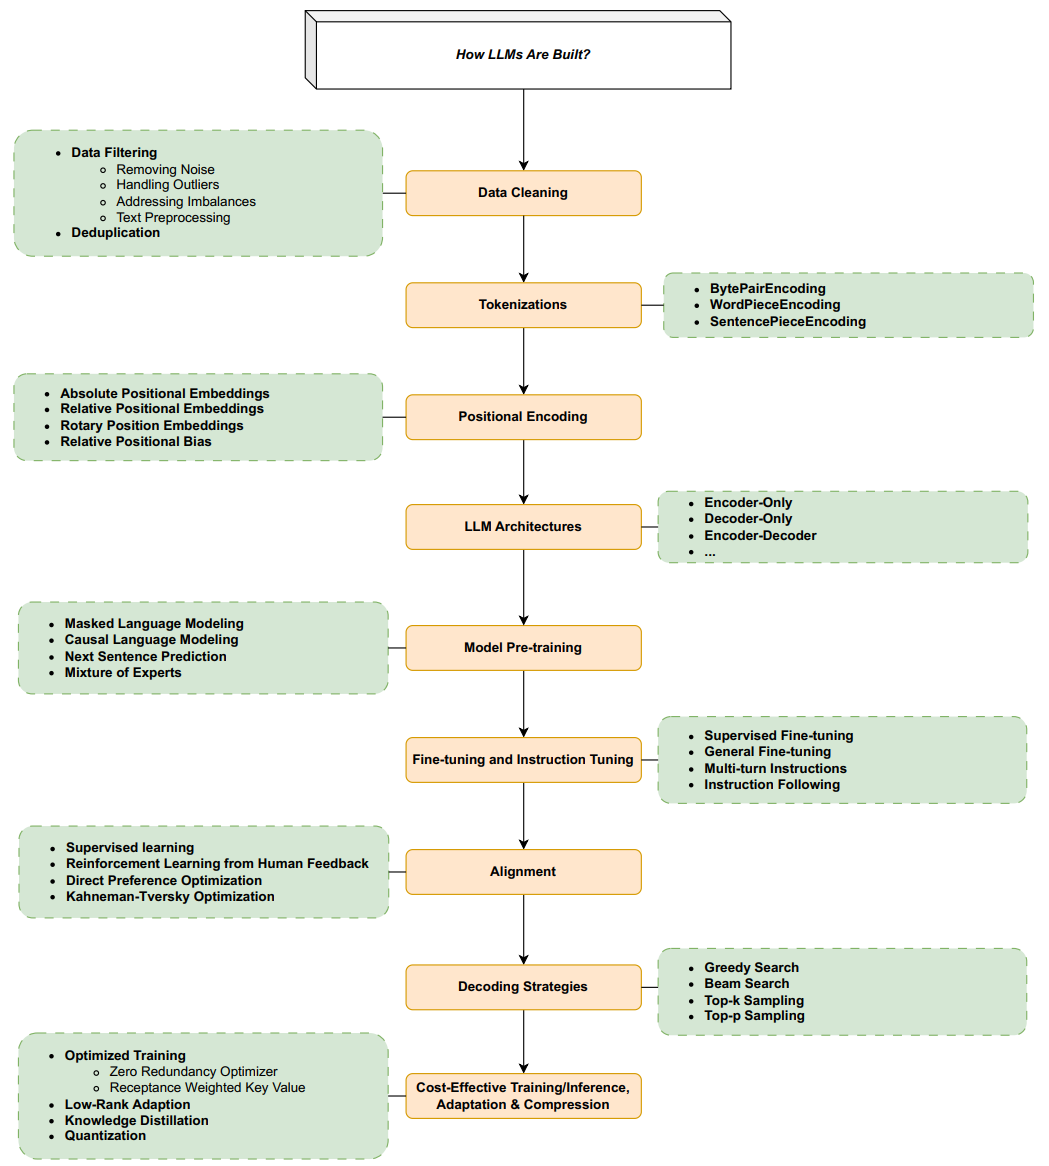
\includegraphics[width=0.90\textwidth]{image/how_llm_works.png}
    \caption{Components of LLMs}
    \label{fig:how_llm_works}
\end{figure}

First we need to deal with data.
\begin{figure}[htbp]
    \centering
    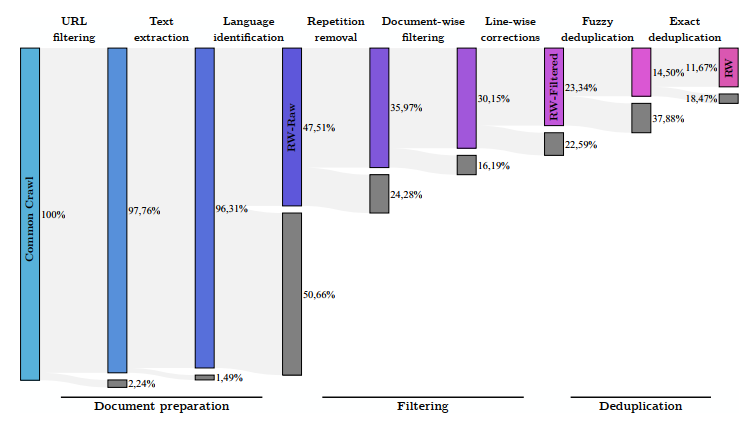
\includegraphics[width=0.80\textwidth]{image/data_process.png}
    \caption{Data Preprocess}
    \label{fig:data_process}
\end{figure}

\begin{itemize}
    \item Data Filtering: Removing the Noise, classifier-based, and heuristic-based frameworks. Handling Outliers. Addressing Imbalances. Text Preprocessing,
removing stop words, punctuation or other elements that may not contribute significantly to the model's learning. Dealing with Ambiguities.
    \item Deduplication: remove duplicate instances, this is important becuase duplicated data will bring biases. The method for this can vary a lot, like 
fuzzy and exact deduplication.
\end{itemize}

\vspace{\baselineskip}

Then we need to tokenize the text.
\begin{itemize}
    \item BytePairEncoding
    \item WordPieceEncoding, start from characters (same as BPE), but when merging, maximize the likelihood of the language model rather than based only on frequncy. 
    \item SentencePieceEncoding, above two assume blank space seperate words, this method start from unicode characters.
\end{itemize}

\vspace{\baselineskip}

Let's we introduce positional encoding.
\begin{itemize}
    \item \mydefination{Absolute Positional Embedding} (APE), drawback is the restriction to a certain number of tokens, and does not count for relative distance.
    \item \mydefination{Relative Positional Embedding} (RPE), add on keys and values.
    \item \mydefination{Rotary Position Embeddings}, used in LLaMA.
    \item \mydefination{Relative Positional Bias}, to facilitate extrapolation during inference.
\end{itemize}

\vspace{\baselineskip}

Model Pre-training:
\begin{itemize}
    \item Autoregressive Language Modeling, $\mathscr L_{ALM}(x) = \sum_{i=1}^N p(x_{i+n} \mid x_i, \ldots, x_{i+n-1})$
    \item Masked Language Modeling, $\mathscr L_{MLM} = \sum_{i=1}^N p(\tilde x \mid x \setminus \tilde x)$
    \item MoE
\end{itemize}

\vspace{\baselineskip}

Fine-tuning and Instruction Tuning. Alignment.
\begin{itemize}
    \item RLHF and RLAIF (reinforcement learning from AI feedback).
    \item DPO (Direct Preference Optimization ), RLHF is complex and unstable. They leveraged a mapping between reward functions and optimal policies to show 
that this constrained reward maximization problem can be optimized exactly with a single stage of policy training, essentially solving a classification 
problem on the human preference data.
    \item Kahneman-Tversky Optimization (KTO), does not need paired preference date $(x, y_w, y_l)$, only need $(x, y)$ and knowledge of whether $y$ is desirable
or undersirable.
\end{itemize}

\begin{figure}[htbp]
    \centering
    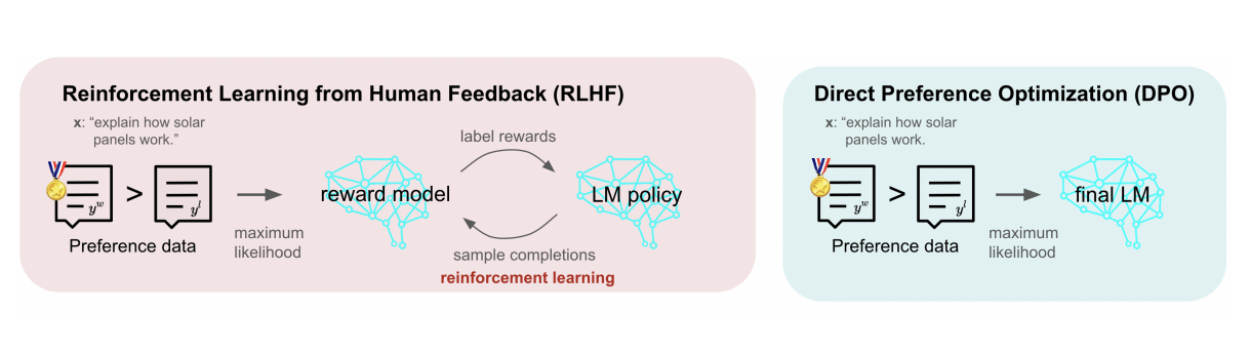
\includegraphics[width=0.80\textwidth]{image/RLHF-vs-DPO.png}
    \caption{RLHF vs DPO}
    \label{fig:RLHF-vs-DPO}
\end{figure}

\begin{figure}[htbp]
    \centering
    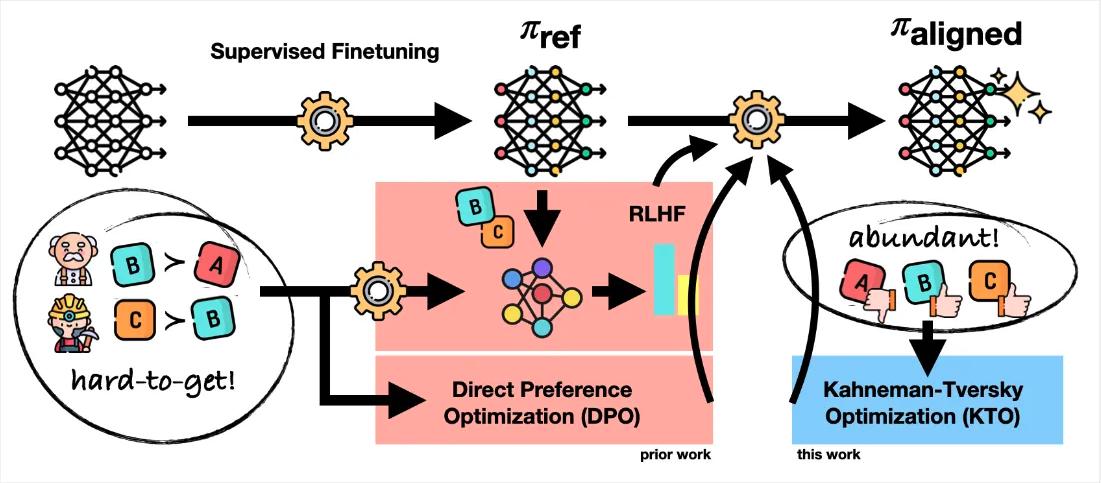
\includegraphics[width=0.80\textwidth]{image/alignment_methods.png}
    \caption{Alignment Methods}
    \label{fig:alignment_methods}
\end{figure}

Decoding Strategies:
\begin{itemize}
    \item Greedy Search, use the most probable token, does not consider the entire sequence.
    \item Beam Search, take $N$ most likely tokens, repeate until max length, and take the maximum total score.
    \item top-k sampling, randomly choose one from k most likely options. $softmax(x_i) = e^{x_i / T} / \sum_j e^{x_j / T}$.
    \item top-p sampling, also known as Nucleus sampling, choose $n$ tokens that $\sum_i^n p(t_i) > P$.
\end{itemize}

\vspace{\baselineskip}

Then we come to cost-efficient training, inference, adaption, compression methods.
\begin{itemize}
    \item Optimized training: Zero Redundancy Optimizer (ZeRO), data- and model-parallel. Receptance Weighted Key Value (RWKV) reformulates the attention 
mechanism to operate in a recurrent fashion, linear time complexity and constant space complexity with respect to sequence length $T$.
    \item Low-Rank Adaption (LoRA)
    \item Knowledge Distillation, response distillation (only mimic outputs), feature distillation (also intermediate layers), API distillation (similar to
response distillation).
    \item Quantization, post training quantization and quantization-aware training.
\end{itemize}

\begin{figure}[htbp]
    \centering
    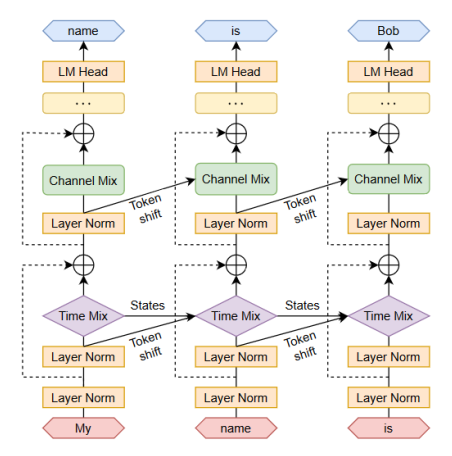
\includegraphics[width=0.50\textwidth]{image/rwkv.png}
    \caption{RWKV architecture}
    \label{fig:rwkv}
\end{figure}

\subsection{How LLMs are used and augmented}

\mydefination{Hallucinations}, categorized into instrinsic and extrinsic hallucination. We can use statistical and model-based matrices to measure it, for 
example, ROUGE, BLEU, PARENT, Knowledge F1 are statistical, IE-Based, QA-Based, NLI-Based and Faithfulness Classification matrics are model-based. And human 
scoring and comparative analysis is also vital. FactScore use both human and model-based, it breaks LLM generation into atomic facts. Ways to mitigate hallucination
are Product Design and User Interaction Strategies, Data Management and Continuous Improvement, Prompt Engineering and Metaprompt Design, Model Selection and Configuration for Hallucination
Mitigation.

\vspace{\baselineskip}

\mydefination{Prompt Engineering} approaches:
\begin{itemize}
    \item \mydefination{Chain of Thought} (CoT), described in \textit{Chain-of-Thought Prompting Elicits Reasoning in Large Language Models}, there are Zero-Shot
CoT (let LLM think step by step) and Manual CoT (give example that shows the reasoning steps, it is better than zero-shot).
    \item Tree of Thought (TOT), first branch out into multiple thought trees than converge, good for complex tasks.
    \item Self-Consistency, generate multiple output and check the consistency, if they are consistent, then these outputs are more likely accurate.
    \item Reflection, let LLM revise its answer.
    \item Expert Prompting, let LLM response as an expert or more experts (which is better).
    \item Chains, \textit{PromptChainer: Chaining Large Language Model Prompts through Visual Programming}, second task depend on first one, create a chain.
    \item Rails, The concept of Rails involves setting up a framework or a set of guidelines that the LLM must follow while generating responses.
    \item Automatic Prompt Engineering (APE), let LLM to generate the prompts, evaluate them and refine them and iterates.
\end{itemize}

\vspace{\baselineskip}

\mydefination{Retrieval Augmented Generation} (RAG): Forward-looking Active Retrieval Augmented Generation
(FLARE) is an advanced RAG that will check the confidence level of the LLM outputs, if it is low, the output will be used as a query to retrieve again, this is
a iterative methods. More details of RAG please refer to \textit{Retrieval-Augmented Generation for Large Language Models: A Survey}.
\begin{figure}[htbp]
    \centering
    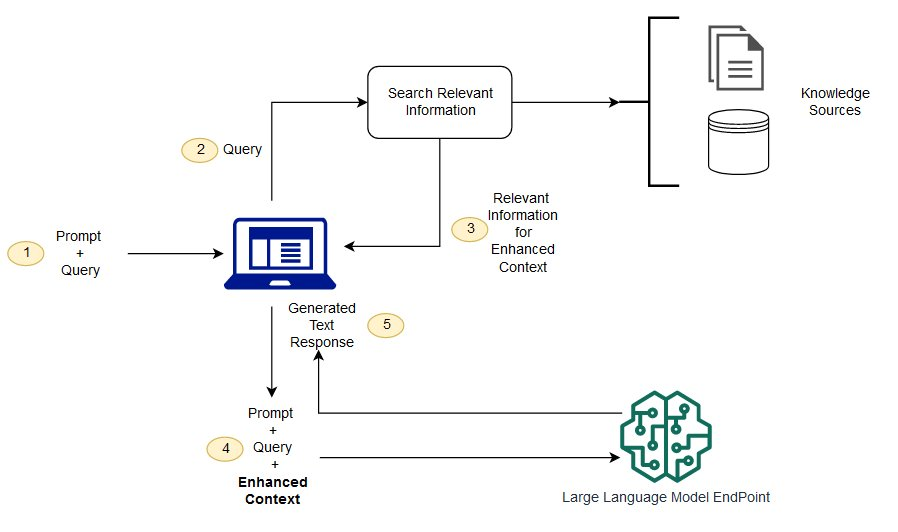
\includegraphics[width=0.75\textwidth]{image/rag.jpg}
    \caption{RAG}
    \label{fig:rag}
\end{figure}

\vspace{\baselineskip}

Then the using of external tools, \textit{Toolformer: Language Models Can Teach Themselves to Use Tools} shows a demo. Automatic Multi-step Reasoning and Tool-use
(ART) involves a systematic approache where, given a task and input, it will search from a task library for the similar task, use it as examples, we can also have
tool library too.

\vspace{\baselineskip}

\mydefination{LLM Agents}: we introduce prompt engineering Techniques for agents, more information please refer to other surveys.
\begin{itemize}
    \item Reasoning without Observation (ReWOO), the LLM initially develops a plan (a series of steps) that outlines
how to approach and solve a given problem. The execution phase then involves integrating actual data or observations into
the pre-specified plan, leading to coherent and contextually relevant responses. This method is good for costly, slow retrieval.
    \item Reason and Act (ReAct), the LLM is prompted to alternate between generating reasoning traces (explanations) and taking
actions (steps or commands) in an interleaved manner.
    \item Dialog-Enabled Resolving Agents (DERA), is developed based on the idea of utilizing multiple agents
within a dialog context, each with specific roles and functions.
\end{itemize}

\subsection{Popular Datasets}
These datasets are \ref{fig:datasets}, and in the paper there is a table for the evaluation metric and links.
\begin{figure}[htbp]
    \centering
    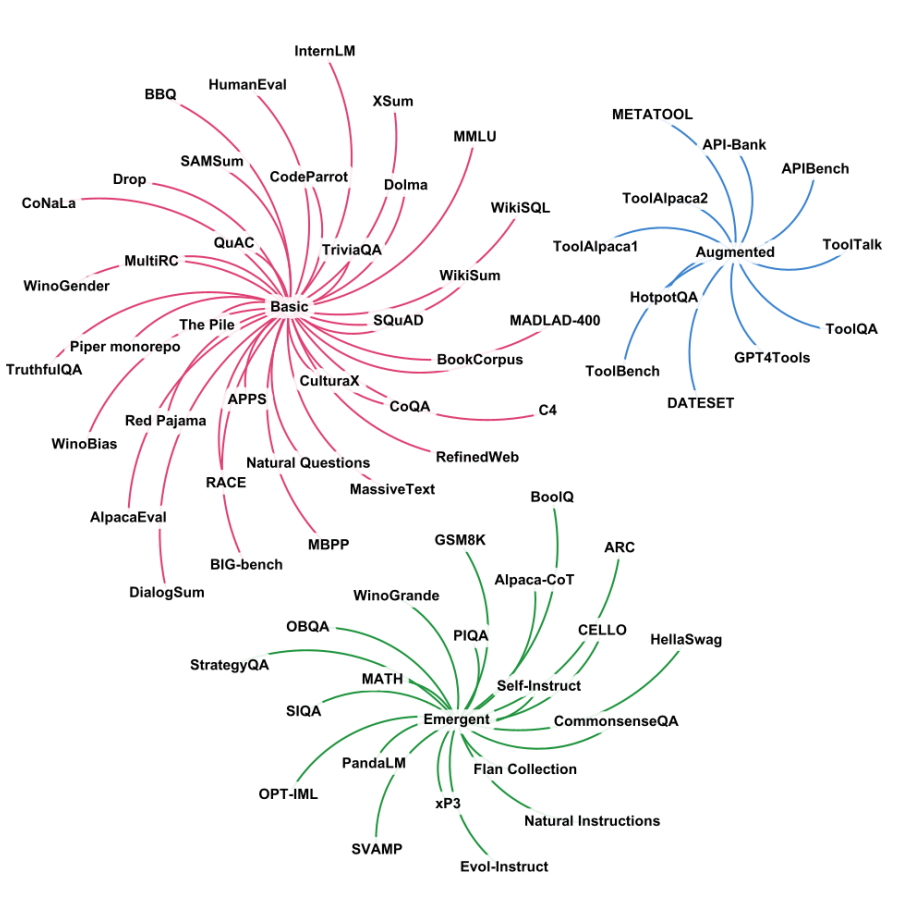
\includegraphics[width=0.75\textwidth]{image/datasets.png}
    \caption{LLM Datesets}
    \label{fig:datasets}
\end{figure}

Evaluation, generate $n$ solution, and if $c$ pass:
\[ \text{pass @} k = \mathbb E_{\text{problems}} \left [ 1 - \frac{\begin{pmatrix} n-c \\ k \end{pmatrix}}{\begin{pmatrix} n \\ k \end{pmatrix}} \right ] \]

\mydefination{Exact Match}, must strictly match the true tokens than it returns 1 else returns 0. \mydefination{Human equivalence score} (HEQ) compare LLM with 
average human accuracy.

\subsection{Challenges and Future}

\begin{enumerate}
    \item Smaller model like Phi from Microsoft, more efficient training like parameter-efficient fine-tuning (PEFT).
    \item New post-attention paradigms, like \mydefination{State Space Models} (SSMs)
    \item Multi-modal LLM
    \item Safe LLM
    \item Agents
\end{enumerate}

\chapter{History Language Models}

\section{Statistical Language Model}

\mydefination{N-Gram} model is the most dominating form of SLMs, which is a Markov chain model, using the statistic from
previous $n-1$ words and current word.
\[ P(w_n \mid w_{n-k}, \ldots, w_{n-1}) = \frac{count(w_{n-k}, \ldots, w_{n})}{count(w_{n-k}, \ldots, w_{n-1})} \]
in n-gram, $k$ is always $n-1$.

In order to deal with unseen words and small probability of larger n-pairs, smooth method are often used, like 
\mydefination{Laplace-smooth}.

\chapter{LLM Techniques}

\section{Model Architecture}

\section{Dataset}

\section{Tokenize}

\section{Positional Encoding}

\mydefination{Relative Positional Embedding}, the attention score is:
\[ e_{ij} = \frac{(q_i + r_{i-j})k_j}{\sqrt{d_k}} \]
where $r_{i-j}$ is an embedding output. Another variants add this to the key or the QK matrix or even to the value matrix.

\mydefination{Rotary Position Embeddings}, let use $R$ for this operation, $q_p, k_p$ are query vector and key vector at position $p$, then attention score is:
\[ \text{score}(q_p, k_p) = \langle R(q_p, p), R(k_p, p) \rangle \]
And $R$ has property: $ \langle R(q, p), R(k, p^{'}) \rangle = \langle R(q, 0), R(k, p^{'} - p) \rangle $.

The math: given $x = [(x_1, x_2), \ldots, (x_{d-1}, x_d)]$, each pair is rotated by an angle $\theta_i \cdot p$, $p$ is the position. 
Let $z_i = x_{2i} + ix_{2i+1}$, $R(z_i,p) = z_i \cdot e^{i\theta_i p}$. The matrix form is:
\[
\begin{bmatrix}
x_{2i}^{'} \\
x_{2i + 1}^{'}
\end{bmatrix}
=
\begin{bmatrix}
\cos(\theta_i p) & -\sin(\theta_i p) \\
\sin(\theta_i p) & -\cos(\theta_i p)
\end{bmatrix}
\begin{bmatrix}
x_{2i} \\
x_{2i + 1}
\end{bmatrix}
\]
RoPE can extrapolate to unseen longer sequences.

\mydefination{Relative Positional Bias}, the math is:
\[ e_{ij} = \frac{q_i k_j}{\sqrt{d_k}} + b_{i-j} \]
for the extrapolation during inference.

\section{Pre-training}

\mydefination{Low-Rank Adaption} (LoRA), $W_0 + \Delta W = W_0 + BA$, where initializations are $A \sim \mathcal N(0, \sigma^2), B=0$. Normally only attention
weight will be adapted, the original weights are frozen.

\end{document}